% Options for packages loaded elsewhere
\PassOptionsToPackage{unicode}{hyperref}
\PassOptionsToPackage{hyphens}{url}
\PassOptionsToPackage{dvipsnames,svgnames,x11names}{xcolor}
\documentclass[
  11pt,
]{article}
\usepackage{xcolor}
\usepackage{amsmath,amssymb}
\setcounter{secnumdepth}{-\maxdimen} % remove section numbering
\usepackage{iftex}
\ifPDFTeX
  \usepackage[T1]{fontenc}
  \usepackage[utf8]{inputenc}
  \usepackage{textcomp} % provide euro and other symbols
\else % if luatex or xetex
  \usepackage{unicode-math} % this also loads fontspec
  \defaultfontfeatures{Scale=MatchLowercase}
  \defaultfontfeatures[\rmfamily]{Ligatures=TeX,Scale=1}
\fi
\usepackage{lmodern}
\ifPDFTeX\else
  % xetex/luatex font selection
\fi
% Use upquote if available, for straight quotes in verbatim environments
\IfFileExists{upquote.sty}{\usepackage{upquote}}{}
\IfFileExists{microtype.sty}{% use microtype if available
  \usepackage[]{microtype}
  \UseMicrotypeSet[protrusion]{basicmath} % disable protrusion for tt fonts
}{}
\makeatletter
\@ifundefined{KOMAClassName}{% if non-KOMA class
  \IfFileExists{parskip.sty}{%
    \usepackage{parskip}
  }{% else
    \setlength{\parindent}{0pt}
    \setlength{\parskip}{6pt plus 2pt minus 1pt}}
}{% if KOMA class
  \KOMAoptions{parskip=half}}
\makeatother
\usepackage{color}
\usepackage{fancyvrb}
\newcommand{\VerbBar}{|}
\newcommand{\VERB}{\Verb[commandchars=\\\{\}]}
\DefineVerbatimEnvironment{Highlighting}{Verbatim}{commandchars=\\\{\}}
% Add ',fontsize=\small' for more characters per line
\usepackage{framed}
\definecolor{shadecolor}{RGB}{248,248,248}
\newenvironment{Shaded}{\begin{snugshade}}{\end{snugshade}}
\newcommand{\AlertTok}[1]{\textcolor[rgb]{0.94,0.16,0.16}{#1}}
\newcommand{\AnnotationTok}[1]{\textcolor[rgb]{0.56,0.35,0.01}{\textbf{\textit{#1}}}}
\newcommand{\AttributeTok}[1]{\textcolor[rgb]{0.13,0.29,0.53}{#1}}
\newcommand{\BaseNTok}[1]{\textcolor[rgb]{0.00,0.00,0.81}{#1}}
\newcommand{\BuiltInTok}[1]{#1}
\newcommand{\CharTok}[1]{\textcolor[rgb]{0.31,0.60,0.02}{#1}}
\newcommand{\CommentTok}[1]{\textcolor[rgb]{0.56,0.35,0.01}{\textit{#1}}}
\newcommand{\CommentVarTok}[1]{\textcolor[rgb]{0.56,0.35,0.01}{\textbf{\textit{#1}}}}
\newcommand{\ConstantTok}[1]{\textcolor[rgb]{0.56,0.35,0.01}{#1}}
\newcommand{\ControlFlowTok}[1]{\textcolor[rgb]{0.13,0.29,0.53}{\textbf{#1}}}
\newcommand{\DataTypeTok}[1]{\textcolor[rgb]{0.13,0.29,0.53}{#1}}
\newcommand{\DecValTok}[1]{\textcolor[rgb]{0.00,0.00,0.81}{#1}}
\newcommand{\DocumentationTok}[1]{\textcolor[rgb]{0.56,0.35,0.01}{\textbf{\textit{#1}}}}
\newcommand{\ErrorTok}[1]{\textcolor[rgb]{0.64,0.00,0.00}{\textbf{#1}}}
\newcommand{\ExtensionTok}[1]{#1}
\newcommand{\FloatTok}[1]{\textcolor[rgb]{0.00,0.00,0.81}{#1}}
\newcommand{\FunctionTok}[1]{\textcolor[rgb]{0.13,0.29,0.53}{\textbf{#1}}}
\newcommand{\ImportTok}[1]{#1}
\newcommand{\InformationTok}[1]{\textcolor[rgb]{0.56,0.35,0.01}{\textbf{\textit{#1}}}}
\newcommand{\KeywordTok}[1]{\textcolor[rgb]{0.13,0.29,0.53}{\textbf{#1}}}
\newcommand{\NormalTok}[1]{#1}
\newcommand{\OperatorTok}[1]{\textcolor[rgb]{0.81,0.36,0.00}{\textbf{#1}}}
\newcommand{\OtherTok}[1]{\textcolor[rgb]{0.56,0.35,0.01}{#1}}
\newcommand{\PreprocessorTok}[1]{\textcolor[rgb]{0.56,0.35,0.01}{\textit{#1}}}
\newcommand{\RegionMarkerTok}[1]{#1}
\newcommand{\SpecialCharTok}[1]{\textcolor[rgb]{0.81,0.36,0.00}{\textbf{#1}}}
\newcommand{\SpecialStringTok}[1]{\textcolor[rgb]{0.31,0.60,0.02}{#1}}
\newcommand{\StringTok}[1]{\textcolor[rgb]{0.31,0.60,0.02}{#1}}
\newcommand{\VariableTok}[1]{\textcolor[rgb]{0.00,0.00,0.00}{#1}}
\newcommand{\VerbatimStringTok}[1]{\textcolor[rgb]{0.31,0.60,0.02}{#1}}
\newcommand{\WarningTok}[1]{\textcolor[rgb]{0.56,0.35,0.01}{\textbf{\textit{#1}}}}
\usepackage{graphicx}
\makeatletter
\newsavebox\pandoc@box
\newcommand*\pandocbounded[1]{% scales image to fit in text height/width
  \sbox\pandoc@box{#1}%
  \Gscale@div\@tempa{\textheight}{\dimexpr\ht\pandoc@box+\dp\pandoc@box\relax}%
  \Gscale@div\@tempb{\linewidth}{\wd\pandoc@box}%
  \ifdim\@tempb\p@<\@tempa\p@\let\@tempa\@tempb\fi% select the smaller of both
  \ifdim\@tempa\p@<\p@\scalebox{\@tempa}{\usebox\pandoc@box}%
  \else\usebox{\pandoc@box}%
  \fi%
}
% Set default figure placement to htbp
\def\fps@figure{htbp}
\makeatother
\setlength{\emergencystretch}{3em} % prevent overfull lines
\providecommand{\tightlist}{%
  \setlength{\itemsep}{0pt}\setlength{\parskip}{0pt}}
% obstruction_preamble.tex — shared house style for ALL papers.
% Engine: pdfLaTeX (portable, no font cache). Injected by pandoc (see makefile).
% pandoc loads fontenc(T1)+inputenc(utf8) before this; hyperref after (so we set
% link colors via pandoc -V flags, not here).

% ---- Fonts & math ----
\IfFileExists{lmodern.sty}{\usepackage{lmodern}}{}   % Latin Modern if present
\usepackage{amsmath,amssymb,amsthm}                  % \mathbb \mathfrak \square ...
\usepackage{microtype}

% ---- Over-wide \boxed kernel statements shrink to fit the text width ----
% A long \boxed{\text{...}} line can exceed \linewidth because \text does not
% line-break in math mode. "max width=\linewidth" scales down ONLY boxes that
% are wider than the text block; short math boxes are left at natural size.
% One place, all papers.
\usepackage{adjustbox}
\let\oboldboxed\boxed
\renewcommand{\boxed}[1]{\adjustbox{max width=\linewidth}{\oboldboxed{#1}}}
\setlength{\emergencystretch}{3em}

% ---- Line breaking for verbatim and code blocks ----
\usepackage{fancyvrb}

% ---- Safe line breaking for typewriter font & long URLs/DOIs ----
\usepackage[htt]{hyphenat}
\usepackage{xurl}
\usepackage[hyphens]{url}


% ---- Flawless fix: literal Unicode (ℓ¹ Φ₁ κ¹ ⊗ →) in TEXT mode ----
% In $...$ these already work; this maps stray text-mode glyphs to math so
% nothing renders blank and you never rewrite source. If a build ever says
% "Unicode character X not set up", add one line here for that glyph.
\usepackage{newunicodechar}
\newcommand{\um}[1]{\ensuremath{#1}}
\newunicodechar{ℓ}{\um{\ell}}
\newunicodechar{Φ}{\um{\Phi}}\newunicodechar{φ}{\um{\varphi}}
\newunicodechar{Ψ}{\um{\Psi}}\newunicodechar{ψ}{\um{\psi}}
\newunicodechar{⇔}{\um{\Leftrightarrow}}
\newunicodechar{Γ}{\um{\Gamma}}\newunicodechar{γ}{\um{\gamma}}
\newunicodechar{Ω}{\um{\Omega}}\newunicodechar{ω}{\um{\omega}}
\newunicodechar{κ}{\um{\kappa}}\newunicodechar{χ}{\um{\chi}}
\newunicodechar{Λ}{\um{\Lambda}}\newunicodechar{λ}{\um{\lambda}}
\newunicodechar{Θ}{\um{\Theta}}\newunicodechar{θ}{\um{\theta}}
\newunicodechar{Δ}{\um{\Delta}}\newunicodechar{δ}{\um{\delta}}
\newunicodechar{Σ}{\um{\Sigma}}\newunicodechar{σ}{\um{\sigma}}
\newunicodechar{Π}{\um{\Pi}}\newunicodechar{π}{\um{\pi}}
\newunicodechar{α}{\um{\alpha}}\newunicodechar{β}{\um{\beta}}
\newunicodechar{ε}{\um{\varepsilon}}\newunicodechar{μ}{\um{\mu}}
\newunicodechar{ρ}{\um{\rho}}\newunicodechar{τ}{\um{\tau}}
\newunicodechar{ν}{\um{\nu}}\newunicodechar{ξ}{\um{\xi}}
\newunicodechar{ζ}{\um{\zeta}}\newunicodechar{η}{\um{\eta}}
\newunicodechar{ℝ}{\um{\mathbb{R}}}\newunicodechar{ℚ}{\um{\mathbb{Q}}}
\newunicodechar{ℤ}{\um{\mathbb{Z}}}\newunicodechar{ℕ}{\um{\mathbb{N}}}
\newunicodechar{ℂ}{\um{\mathbb{C}}}
\newunicodechar{𝒟}{\um{\mathcal{D}}}
\newunicodechar{→}{\um{\to}}\newunicodechar{↦}{\um{\mapsto}}
\newunicodechar{≤}{\um{\leq}}\newunicodechar{≥}{\um{\geq}}
\newunicodechar{≠}{\um{\neq}}\newunicodechar{≈}{\um{\approx}}
\newunicodechar{≅}{\um{\cong}}\newunicodechar{≡}{\um{\equiv}}
\newunicodechar{⊗}{\um{\otimes}}\newunicodechar{⊕}{\um{\oplus}}
\newunicodechar{∘}{\um{\circ}}\newunicodechar{∂}{\um{\partial}}
\newunicodechar{∇}{\um{\nabla}}\newunicodechar{∑}{\um{\sum}}
\newunicodechar{∏}{\um{\prod}}\newunicodechar{∞}{\um{\infty}}
\newunicodechar{⊆}{\um{\subseteq}}\newunicodechar{⊂}{\um{\subset}}
\newunicodechar{⊇}{\um{\supseteq}}\newunicodechar{∈}{\um{\in}}
\newunicodechar{∉}{\um{\notin}}\newunicodechar{∩}{\um{\cap}}
\newunicodechar{∪}{\um{\cup}}\newunicodechar{∖}{\um{\setminus}}
\newunicodechar{∅}{\um{\varnothing}}\newunicodechar{⊥}{\um{\perp}}
\newunicodechar{∀}{\um{\forall}}\newunicodechar{∃}{\um{\exists}}
\newunicodechar{±}{\um{\pm}}\newunicodechar{×}{\um{\times}}\newunicodechar{−}{\um{-}}
\newunicodechar{·}{\um{\cdot}}\newunicodechar{√}{\um{\surd}}
\newunicodechar{⟨}{\um{\langle}}\newunicodechar{⟩}{\um{\rangle}}
\newunicodechar{≪}{\um{\ll}}\newunicodechar{≫}{\um{\gg}}
\newunicodechar{∝}{\um{\propto}}\newunicodechar{≜}{\um{\triangleq}}
\newunicodechar{⇒}{\um{\Rightarrow}}\newunicodechar{⇐}{\um{\Leftarrow}}
\newunicodechar{∧}{\um{\wedge}}\newunicodechar{∨}{\um{\vee}}
\newunicodechar{⟺}{\um{\iff}}\newunicodechar{□}{\um{\square}}
\newunicodechar{⊔}{\um{\sqcup}}\newunicodechar{…}{\dots}\newunicodechar{‖}{\um{\Vert}}
\newunicodechar{▼}{\um{\blacktriangledown}}\newunicodechar{«}{\guillemotleft}\newunicodechar{»}{\guillemotright}
\newunicodechar{─}{--}\newunicodechar{│}{|}\newunicodechar{┌}{+}\newunicodechar{┐}{+}\newunicodechar{┼}{+}
\newunicodechar{═}{=}\newunicodechar{║}{\um{\parallel}}\newunicodechar{̄}{\={}}
\newunicodechar{⟹}{\um{\implies}}\newunicodechar{⟸}{\um{\impliedby}}
\newunicodechar{⁰}{\textsuperscript{0}}\newunicodechar{¹}{\textsuperscript{1}}
\newunicodechar{²}{\textsuperscript{2}}\newunicodechar{³}{\textsuperscript{3}}
\newunicodechar{⁴}{\textsuperscript{4}}\newunicodechar{⁵}{\textsuperscript{5}}
\newunicodechar{⁶}{\textsuperscript{6}}\newunicodechar{⁷}{\textsuperscript{7}}
\newunicodechar{⁸}{\textsuperscript{8}}\newunicodechar{⁹}{\textsuperscript{9}}
\newunicodechar{⁻}{\textsuperscript{-}}\newunicodechar{⁺}{\textsuperscript{+}}
\newunicodechar{ⁿ}{\textsuperscript{n}}
\newunicodechar{₀}{\textsubscript{0}}\newunicodechar{₁}{\textsubscript{1}}\newunicodechar{ᵀ}{\textsuperscript{T}}
\newunicodechar{₂}{\textsubscript{2}}\newunicodechar{₃}{\textsubscript{3}}
\newunicodechar{₄}{\textsubscript{4}}\newunicodechar{₅}{\textsubscript{5}}\newunicodechar{⋯}{\um{\cdots}}
\newunicodechar{ₜ}{\textsubscript{t}}\newunicodechar{ₑ}{\textsubscript{e}}\newunicodechar{ₙ}{\textsubscript{n}}

% ---- Geometry & spacing ----
\usepackage{geometry}\geometry{letterpaper,margin=1in}
\setlength{\parindent}{0pt}\setlength{\parskip}{0.55\baselineskip}\linespread{1.04}

% ---- Palette ----
\usepackage{xcolor}
\definecolor{oblink}{HTML}{1A4D8F}\definecolor{obrule}{HTML}{C2CCD6}
\definecolor{obboxbg}{HTML}{F6F8FA}
\definecolor{obproven}{HTML}{1B7F4B}   % PROVEN / DERIVED / STANDARD
\definecolor{obconj}{HTML}{B45309}     % CONJECTURE / OPEN / FALSE
\definecolor{obdef}{HTML}{6B21A8}      % DEFINITION / INTERPRETIVE
\definecolor{obneutral}{HTML}{475569}

% ---- Headings ----
\usepackage{titlesec}
\titleformat{\section}{\Large\bfseries}{\thesection}{0.6em}{}
\titleformat{\subsection}{\large\bfseries}{\thesubsection}{0.6em}{}
\titleformat{\subsubsection}{\normalsize\bfseries}{\thesubsubsection}{0.6em}{}
\titlespacing*{\section}{0pt}{1.4em}{0.5em}
\titlespacing*{\subsection}{0pt}{1.1em}{0.4em}

% ---- Theorem environments (for when you adopt semantic theorems) ----
\theoremstyle{plain}
\newtheorem{theorem}{Theorem}[section]
\newtheorem{lemma}[theorem]{Lemma}
\newtheorem{proposition}[theorem]{Proposition}
\newtheorem{corollary}[theorem]{Corollary}
\newtheorem{conjecture}[theorem]{Conjecture}
\theoremstyle{definition}\newtheorem{definition}[theorem]{Definition}
\theoremstyle{remark}\newtheorem*{remark}{Remark}

% ---- Blockquotes -> one uniform left-ruled callout ----
% pandoc wraps every `>` block (your theorems, Status notes, caveats) in `quote`.
\usepackage{mdframed}
\renewenvironment{quote}{%
  \begin{mdframed}[linewidth=0pt,leftline=true,linecolor=obrule,
    rightline=false,topline=false,bottomline=false,
    innerleftmargin=1em,innerrightmargin=0.8em,innertopmargin=0.5em,
    innerbottommargin=0.5em,skipabove=0.6em,skipbelow=0.6em,
    backgroundcolor=obboxbg]\small}{\end{mdframed}}

% ---- Claim-type tag macro ----
\newcommand{\claimtag}[2]{{\small\sffamily\bfseries\color{#1}[#2]}}

% ---- Inline code / file references -> standard breakable typewriter font ----
\DeclareRobustCommand{\texttt}[1]{%
  \ifmmode
    \mathtt{#1}%
  \else
    {\ttfamily\small\renewcommand{\_}{\symbol{95}\allowbreak}#1}%
  \fi}



% ---- "What this does not claim" box ----
\usepackage[most]{tcolorbox}
\newtcolorbox{nonclaim}{colback=obboxbg,colframe=obrule,boxrule=0.6pt,arc=2pt,
  left=1em,right=1em,top=0.5em,bottom=0.5em,
  title={What this does not claim},fonttitle=\bfseries,
  coltitle=black,colbacktitle=obboxbg}

% ---- Tables ----
\usepackage{booktabs}\renewcommand{\arraystretch}{1.15}
\usepackage{etoolbox}
% Compact tables, and let over-long \mathsf{CamelCase} status identifiers wrap
% inside cells. In math, \mathsf{ContinuumShadowBecomesFakeAuthority} is a single
% unbreakable atom and overruns narrow pandoc columns. Scoped to tables only, we
% re-render \mathsf as a sequence of per-word \mathsf atoms split before each
% interior capital and joined by \allowbreak, so the identifier wraps at the math
% top level (an \allowbreak between atoms IS a legal break in inline math; a text
% \mbox/\seqsplit is not). Also shrink the table font and tighten column padding.
% Body math is untouched; table cells carry only plain ASCII identifiers, so the
% splitter is emoji-safe. One place, all papers.
\let\obmathsforig\mathsf
\ExplSyntaxOn
\tl_new:N \l__obt_run_tl
\int_new:N \l__obt_i_int
\cs_new_protected:Npn \__obt_emit:
  {
    \tl_if_empty:NF \l__obt_run_tl
      {
        \int_compare:nNnT { \l__obt_i_int } > { 1 } { \allowbreak }
        \exp_args:NV \obmathsforig \l__obt_run_tl
        \int_incr:N \l__obt_i_int
        \tl_clear:N \l__obt_run_tl
      }
  }
\cs_new_protected:Npn \obtablesf #1
  {
    \tl_clear:N \l__obt_run_tl
    \int_set:Nn \l__obt_i_int { 1 }
    \tl_map_inline:nn {#1}
      {
        \str_if_eq:eeT { \str_uppercase:n {##1} } {##1}
          { \str_if_eq:eeF { \str_lowercase:n {##1} } {##1} { \__obt_emit: } }
        \tl_put_right:Nn \l__obt_run_tl {##1}
      }
    \__obt_emit:
  }
\ExplSyntaxOff
\AtBeginEnvironment{longtable}{\small\setlength{\tabcolsep}{4pt}\let\mathsf\obtablesf}
\AtBeginEnvironment{tabular}{\let\mathsf\obtablesf}

% ---- Title block polish (pandoc \maketitle) ----
% Title and subtitle both centered under each other. Body metadata stays plain
% roman (never a monospaced identity dump). Public monographs must not put
% internal programme IDs (PO-xxx, GS-xxx, …) in the title line.
\usepackage{titling}
\newcommand{\obsubtitle}{}
% Capture pandoc's \subtitle{...} (provide later is a no-op once this is defined).
\newcommand{\subtitle}[1]{\gdef\obsubtitle{#1}}
\pretitle{\begin{center}\LARGE\bfseries}
\posttitle{%
  \par
  \ifx\obsubtitle\empty\else
    \vskip0.4em
    {\large\itshape \obsubtitle\par}%
  \fi
  \end{center}\vskip0.75em}
\preauthor{\begin{center}\large}\postauthor{\par\end{center}}
\predate{\begin{center}\normalsize}\postdate{\par\end{center}\vskip0.5em\hrule\vskip1em}

% ---- Status-box markers (emoji rendered as text glyphs; one place, all papers) ----
\newunicodechar{§}{\S}
\newunicodechar{–}{--}
\newunicodechar{—}{---}
\newunicodechar{‘}{`}
\newunicodechar{’}{'}
\newunicodechar{“}{``}
\newunicodechar{”}{''}
\newunicodechar{✅}{\um{\checkmark}}
\newunicodechar{⚠}{\textbf{!}}
\newunicodechar{☣}{\um{\boxtimes}}
\newunicodechar{⊣}{\um{\dashv}}
\newunicodechar{🔷}{\textcolor{oblink}{\um{\blacklozenge}}}
\newunicodechar{️}{}
\usepackage{bookmark}
\IfFileExists{xurl.sty}{\usepackage{xurl}}{} % add URL line breaks if available
\urlstyle{same}
\hypersetup{
  pdftitle={Blind Spots Under Nonlinear Aggregation and Adjoint Probing},
  pdfauthor={Jeremy H. Carroll},
  pdfkeywords={observation operator, kernel, nonlinear aggregation, Gram operator, adjoint probing, singular values, Lean 4},
  colorlinks=true,
  linkcolor={oblink},
  filecolor={Maroon},
  citecolor={oblink},
  urlcolor={oblink},
  pdfcreator={LaTeX via pandoc}}

\author{}
\date{2026-10-15}

\begin{document}

\section{Blind Spots Under Nonlinear Aggregation and Adjoint Probing}\label{blind-spots-under-nonlinear-aggregation-and-adjoint-probing}

\textbf{Author:} Jeremy H. Carroll

\textbf{Date:} 2026-10-15

\textbf{Version:} 0.1.1

\subsection{Abstract}\label{abstract}

Let a finite family of evaluators be represented by one stacked real matrix

\[
Q:\mathbb{R}^{d}\longrightarrow\mathbb{R}^{m}.
\]

The local report is \(Qx\). Any deterministic rule applied only after this
report---thresholding, voting, ranking, or another nonlinear map---receives the
same input on states \(x\) and \(y\) whenever \(Qx=Qy\). It therefore cannot
separate them. In particular, a rule that accepts the zero report also accepts
every state in \(\ker Q\).

The positive result is equally small. The Gram operator
\(H=Q^{\mathsf T}Q\) vanishes exactly on \(\ker Q\). Centered directional
evaluations of the quadratic energy \(f(x)=\tfrac12\lVert Qx\rVert_2^2\)
recover pairings with \(Hx\); averaging over the full sign cube recovers
\(Hx\) itself. These facts give a finite, testable account of observation
blind spots and adjoint probes. The package includes a self-contained Python
implementation, Lean proofs of the rational Gram identity and the two probe
identities, two executable notebooks, and an injected watcher mutation that
must be detected and then recovered.

\subsection{1. The picture before the notation}\label{the-picture-before-the-notation}

Consider

\[
Q=\begin{bmatrix}1&0\end{bmatrix}.
\]

The evaluator sees the horizontal coordinate and ignores the vertical one.
Every state \((0,t)\) produces the report \(0\), regardless of \(t\). Sending
that report through a majority vote or a complicated ranking model does not
reveal the missing coordinate: the downstream rule still receives \(0\).

\begin{figure}
\centering
\pandocbounded{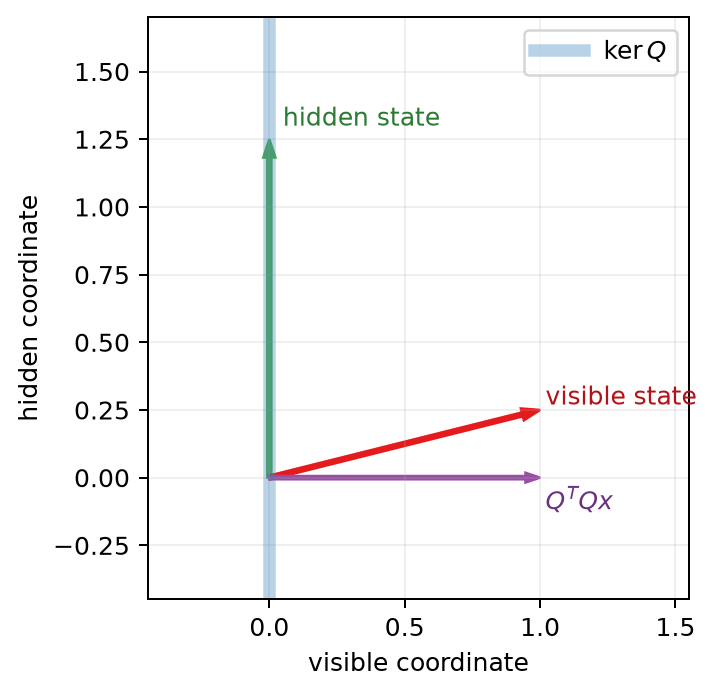
\includegraphics[keepaspectratio,alt={A hidden direction and its visible adjoint response}]{figures/figure_1_kernel_and_adjoint.png}}
\caption{A hidden direction and its visible adjoint response}
\end{figure}

The blue axis in Figure 1 is \(\ker Q\). A vector on that axis is hidden. A
vector with a horizontal component is visible, and \(Q^{\mathsf T}Qx\) points
in the visible subspace. This two-dimensional diagram is the whole argument
in miniature.

\subsection{2. Observation-only decisions}\label{observation-only-decisions}

Let \(Q\in\mathbb{R}^{m\times d}\). The stacked report of a state
\(x\in\mathbb{R}^{d}\) is

\[
O(x)=Qx.
\]

A deterministic postprocessor is any function
\(A:\mathbb{R}^{m}\to\mathcal V\), where \(\mathcal V\) is a set of verdicts.
No continuity, linearity, or monotonicity is assumed.

\subsubsection{Theorem 1: postprocessing invariance}\label{theorem-1-postprocessing-invariance}

If \(Qx=Qy\), then

\[
A(Qx)=A(Qy).
\]

\textbf{Proof.} Substitute the equal arguments into the function \(A\). \(\square\)

The theorem is elementary, but it locates the information boundary precisely:
nonlinearity after observation cannot reconstruct a coordinate discarded by
observation.

\subsubsection{Corollary 1: zero-preserving aggregation}\label{corollary-1-zero-preserving-aggregation}

Suppose a distinguished verdict \(\mathsf{green}\in\mathcal V\) satisfies
\(A(0)=\mathsf{green}\). Then every \(x\in\ker Q\) receives
\(\mathsf{green}\).

This includes a threshold rule, unanimous voting on zero local scores, and a
\(k\)-of-\(n\) rule when all local scores vanish. It says nothing about rules
that inspect the original state or make an additional observation.

\subsubsection{Theorem 2: the accepted cylinder}\label{theorem-2-the-accepted-cylinder}

Assume \(Q\neq 0\) and \(\tau\geq 0\). Let \(\sigma_{\min}^{+}(Q)\) be its least positive
singular value. If

\[
\lVert Qx\rVert_2\leq \tau,
\]

then

\[
\operatorname{dist}(x,\ker Q)
\leq \frac{\tau}{\sigma_{\min}^{+}(Q)}.
\]

\textbf{Proof.} Write \(x=k+u\) using the orthogonal decomposition
\(\mathbb R^d=\ker Q\oplus(\ker Q)^\perp\). Then \(Qx=Qu\), and the singular
value bound on \((\ker Q)^\perp\) gives

\[
\lVert Qx\rVert_2=\lVert Qu\rVert_2
\geq \sigma_{\min}^{+}(Q)\lVert u\rVert_2.
\]

Because \(\lVert u\rVert_2=\operatorname{dist}(x,\ker Q)\), division yields
the result. \(\square\)

This singular-value argument is cited from classical Euclidean matrix analysis {[}1{]}.
The package does not mechanize real singular
values in Lean 4, and the floating-point helper \texttt{cylinder\_radius} is not this
argument. The zero operator is excluded because it has no positive singular
value and its accepted set is all of \(\mathbb R^d\).

\subsection{3. The adjoint signal}\label{the-adjoint-signal}

Define

\[
H=Q^{\mathsf T}Q.
\]

\subsubsection{Theorem 3: Gram kernel identity}\label{theorem-3-gram-kernel-identity}

For every finite real matrix \(Q\),

\[
\ker H=\ker Q.
\]

Consequently,

\[
Hx\neq 0\quad\Longleftrightarrow\quad Qx\neq 0.
\]

The classical real-matrix sentence
\(\operatorname{range}(H)=(\ker Q)^\perp\)
is recorded here and is not part of the mechanized statement.

\textbf{Proof.} If \(Qx=0\), then \(Hx=Q^{\mathsf T}Qx=0\). Conversely, if
\(Hx=0\), then

\[
0=x^{\mathsf T}Hx=x^{\mathsf T}Q^{\mathsf T}Qx
=\lVert Qx\rVert_2^2,
\]

so \(Qx=0\). Thus the kernels agree. \(\square\)

Lean formalizes that identity for every finite rational matrix (\texttt{lean4/Core.lean} {[}3{]}), together with the
equivalent statement that the Gram response is nonzero exactly on detectable
states. The further sentence \(\operatorname{range}(H)=(\ker Q)^\perp\), which
uses the orthogonal complement of a real kernel, is outside the rational Lean
formalization.

This result does not make a hidden state visible: if \(x\in\ker Q\), then
\(Hx=0\). It identifies the response produced by a state that already has a
detectable component and supplies an operator for selecting visible probe
directions.

\subsection{4. Two-query and sign probes}\label{two-query-and-sign-probes}

Set

\[
f(x)=\frac12\lVert Qx\rVert_2^2=\frac12x^{\mathsf T}Hx.
\]

\subsubsection{Theorem 4: centered directional identity}\label{theorem-4-centered-directional-identity}

For every \(c>0\) and direction \(d\),

\[
\frac{f(x+cd)-f(x-cd)}{2c}=d^{\mathsf T}Hx.
\]

\textbf{Proof.} Expand both quadratic forms. The \(x^{\mathsf T}Hx\) and
\(c^2d^{\mathsf T}Hd\) terms cancel; symmetry of \(H\) leaves
\(2c\,d^{\mathsf T}Hx\) in the numerator. \(\square\)

Thus two evaluations of \(f\) measure one pairing with the adjoint signal.

\subsubsection{Theorem 5: full sign-cube recovery}\label{theorem-5-full-sign-cube-recovery}

Let \(\delta\) range uniformly over \(\{-1,+1\}^{d}\), and define

\[
\widehat g(\delta)
=\left(\frac{f(x+c\delta)-f(x-c\delta)}{2c}\right)\delta.
\]

Then

\[
\mathbb E_{\delta}[\widehat g(\delta)]=Hx.
\]

\textbf{Proof.} Theorem 4 gives

\[
\widehat g(\delta)=\delta\delta^{\mathsf T}Hx.
\]

Across the full sign cube, diagonal products are \(1\), while each
off-diagonal product is \(+1\) for half the signs and \(-1\) for half. Hence
\(\mathbb E[\delta\delta^{\mathsf T}]=I\), which establishes the identity.
\(\square\)

\begin{figure}
\centering
\pandocbounded{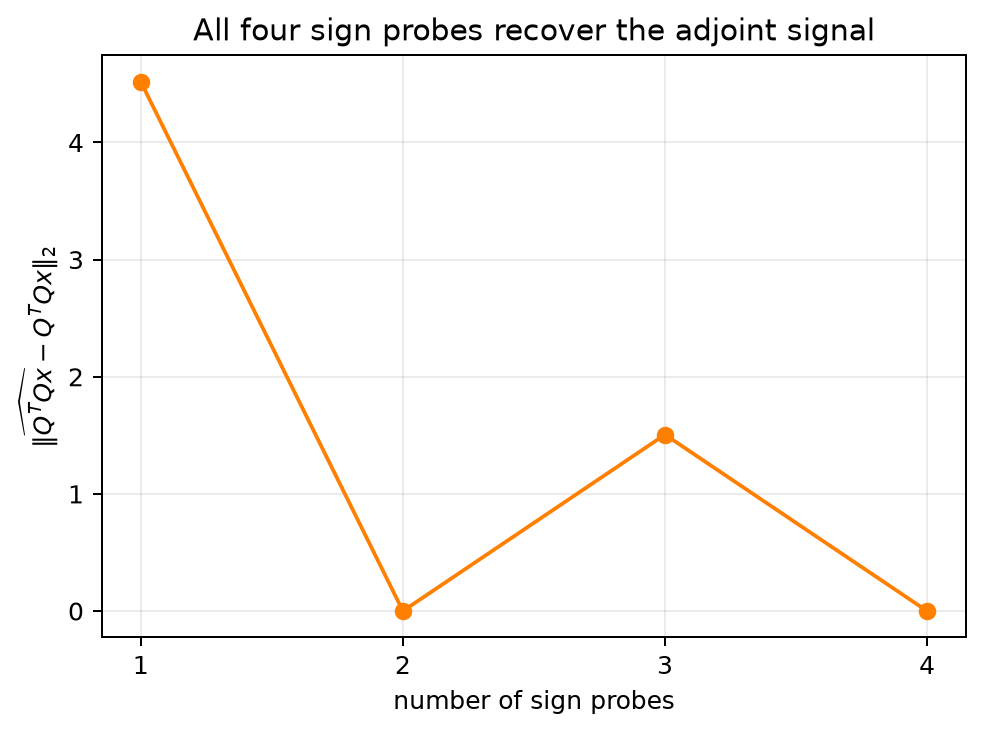
\includegraphics[keepaspectratio,alt={Finite sign-probe error}]{figures/figure_2_sign_probe_error.png}}
\caption{Finite sign-probe error}
\end{figure}

Figure 2 shows a two-dimensional ordering of the four signs. Intermediate
prefixes need not be accurate; the full average is exact up to floating-point
roundoff. A random finite subset is an estimator with sampling error. No
optimization-rate or live-model claim follows from this finite identity. The
construction is related to simultaneous perturbation methods {[}2{]}.

\subsection{5. Executable falsification}\label{executable-falsification}

The reference fixture uses

\[
Q_0=\begin{bmatrix}1&0\end{bmatrix},
\qquad
k=\begin{bmatrix}0\\1\end{bmatrix}.
\]

It checks three ordered facts:

\begin{enumerate}
\def\labelenumi{\arabic{enumi}.}
\tightlist
\item
  baseline: \(Q_0k=0\);
\item
  break: replacing the second matrix entry by \(0.25\) makes the observation
  nonzero;
\item
  recovery: restoring the entry to zero restores \(Q_0k=0\).
\end{enumerate}

The test is useful because it demonstrates that the check can fail for a targeted bad
input. It is one finite falsifier, not an estimate of mutation-detection power.

The Python package also validates dimensions and finite values, computes SVD
bases and cylinder radii, evaluates zero-preserving aggregators, runs Gram
power iteration, generates both figures, and rejects malformed probe inputs.

\subsection{6. What Lean mechanizes}\label{what-lean-mechanizes}

\texttt{lean4/Core.lean} formalizes these statements.

\begin{enumerate}
\def\labelenumi{\arabic{enumi}.}
\tightlist
\item
  Deterministic postprocessing preserves an equality of observations.
\item
  Zero-preserving postprocessing accepts a state with the zero observation.
\item
  Where a \texttt{GramSystem} assumes the kernel identity, hidden states are exactly
  the zero Gram response, and a detectable state has nonzero Gram response.
\item
  For every finite rational matrix, the Gram response is zero exactly when
  the observation is zero.
\item
  The centered two-query derivative equals the Gram pairing for every nonzero
  rational step.
\item
  The average of that probe over the full sign cube recovers each coordinate
  of the Gram response.
\end{enumerate}

The Euclidean cylinder bound in Theorem 2 and the orthogonal-range statement in
Theorem 3 are classical real-matrix results outside the rational Lean formalization.
Exact rational Python checks call the shipped Fraction functions on the paper
fixture and on one nonsingular step. \texttt{check\_axioms.lean} prints the dependency
report for the mechanized declarations. \texttt{lean4/AXIOM\_REPORT.txt} records a
deterministic source-bound rendering of a fresh elaboration; the release
verifier recaptures and compares it.

\subsection{7. Learning path}\label{learning-path}

The two notebooks are the public interactive face of the package.

\begin{itemize}
\tightlist
\item
  \texttt{01\_observation\_blind\_spots.ipynb} starts with shadows and hidden motion,
  then builds \(Q\), \(\ker Q\), nonlinear verdicts, the SVD cylinder, and the
  proof of Theorems 1--3. Sliders vary visible and hidden coordinates.
\item
  \texttt{02\_adjoint\_probes\_and\_falsifiers.ipynb} derives Theorems 4--5, visualizes
  sign-probe error, runs the watcher mutation, and ends with research-level
  questions about noisy or adaptive observations. A widget varies the probe
  prefix length.
\end{itemize}

Both notebooks execute from a clean kernel in the test suite; their committed
outputs are empty.

\subsection{8. Disposition of the former omnibus}\label{disposition-of-the-former-omnibus}

The former manuscript combined the finite theorems above with cached or live
language-model experiments, repository fixtures, distributed communication,
Byzantine behavior, transformer dynamics, Lie-group examples, and sheaf
models. Those subjects require different assumptions and evidence. They are
not absorbed into this paper.

Earlier exploratory prototypes and receipts from the preliminary omnibus lineage
are excluded from this release. \texttt{docs/research\_program\_25\_steps.md} assigns each
deferred topic an artifact and an acceptance test. A later paper may cite a
result only after the corresponding steps are satisfied with current evidence.

\subsection{9. Scope}\label{scope}

This paper establishes finite real-matrix statements and reports deterministic
fixtures. It does not evaluate a language model, certify a software or social
system, establish convergence of a stochastic optimizer, or demonstrate the
distributed, adversarial, transformer, Lie-group, or sheaf extensions in the
research program.

\subsection{10. Reproduction}\label{reproduction}

From the package root, install the declared development dependencies and run
the release verifier:

\begin{Shaded}
\begin{Highlighting}[]
\NormalTok{uv run {-}{-}isolated {-}{-}frozen {-}{-}extra dev python verify\_deposit.py {-}{-}lean}
\end{Highlighting}
\end{Shaded}

It runs the full Python suite over eight workers, requires at least 95\% line
and 95\% branch coverage separately for each production module, rebuilds the
TeX and PDF twice with pdfLaTeX, builds the dated archive twice, and performs a
short-path Lean build and theorem-level axiom census.

To refresh producer outputs before regenerating the manifests:

\begin{Shaded}
\begin{Highlighting}[]
\NormalTok{uv run {-}{-}isolated {-}{-}frozen {-}{-}extra dev python code/generate\_figures.py}
\NormalTok{uv run {-}{-}isolated {-}{-}frozen {-}{-}extra dev python scripts/capture\_axiom\_report.py}
\NormalTok{uv run {-}{-}isolated {-}{-}frozen {-}{-}extra dev python scripts/build\_paper\_artifacts.py}
\NormalTok{uv run {-}{-}isolated {-}{-}frozen {-}{-}extra dev python scripts/regen\_sha256sums.py}
\NormalTok{uv run {-}{-}isolated {-}{-}frozen {-}{-}extra dev python scripts/build\_deposit\_zip.py}
\end{Highlighting}
\end{Shaded}

The paper producer verifies the live shared-preamble hash, runs pdfLaTeX
exactly twice, leaves sections unnumbered, and writes a layout log under
\texttt{dist/}. The archive name carries the paper identifier and release date. The
release manifest pins the paper, code, notebooks, figures, bundled preamble,
axiom report, and proof sources.

\subsection{References}\label{references}

\begin{enumerate}
\def\labelenumi{\arabic{enumi}.}
\tightlist
\item
  G. H. Golub and C. F. Van Loan, \emph{Matrix Computations}, fourth edition,
  Johns Hopkins University Press, 2013.
  \href{https://doi.org/10.56021/9781421407944}{doi:10.56021/9781421407944}
\item
  J. C. Spall, ``Multivariate stochastic approximation using a simultaneous
  perturbation gradient approximation,'' \emph{IEEE Transactions on Automatic
  Control} 37(3), 332--341, 1992.
  \href{https://doi.org/10.1109/9.119632}{doi:10.1109/9.119632}
\item
  L. de Moura and S. Ullrich, ``The Lean 4 theorem prover and programming
  language,'' \emph{Automated Deduction---CADE 28}, Lecture Notes in Computer Science,
  vol.~12699, 625--635, 2021.
  \href{https://doi.org/10.1007/978-3-030-79876-5_37}{doi:10.1007/978-3-030-79876-5\_37}
\end{enumerate}

\end{document}
